% exercise sheet with header on every page for math or close subjects
\documentclass[12pt]{article}
\usepackage[utf8]{inputenc}
\usepackage{latexsym}
\usepackage{multicol}
\usepackage{fancyhdr}
\usepackage{amsfonts}
\usepackage{amsmath}
\usepackage{amssymb}
\usepackage{enumerate}
\usepackage{listings}
\usepackage{graphicx}
\usepackage[parfill]{parskip}

% Shortcuts for bb, frak and cal letters
\newcommand{\E}{\mathbb{E}}
\newcommand{\V}{\mathbb{V}}
\renewcommand{\P}{\mathbb{P}}
\newcommand{\N}{\mathbb{N}}
\newcommand{\R}{\mathbb{R}}
\newcommand{\C}{\mathbb{C}}
\newcommand{\Z}{\mathbb{Z}}
\newcommand{\Pfrak}{\mathfrak{P}}
\newcommand{\Pfrac}{\mathfrak{P}}
\newcommand{\Bfrac}{\mathfrak{P}}
\newcommand{\Bfrak}{\mathfrak{B}}
\newcommand{\Fcal}{\mathcal{F}}
\newcommand{\Ycal}{\mathcal{Y}}
\newcommand{\Bcal}{\mathcal{B}}
\newcommand{\Acal}{\mathcal{A}}

% formating
\topmargin -3.5cm
\textheight 22cm
\textwidth 16.0 cm
\oddsidemargin -0.1cm

% Fancy Header on every Page
\pagestyle{fancy}
\lhead{\textbf{Embedded Systems Problem Set F}}
\rhead{Daniel Schäfer (2549458) \\ Kevin M\"uller (2550062) \\ Rafael Dewes (2548365) }
\renewcommand{\headrulewidth}{1.2pt}
\setlength{\headheight}{110pt}

\begin{document}
\pagenumbering{gobble}
\lstset{language=C++}

\section*{Problem F1}
\subsection*{a)}
In contrast to DFA's Büchi Automata take infinite input sequences. To be an accepted input by the automaton there has to be a run of the sequence that includes an accepting state an infinite amount of times. 
They accept omega regular languages whereas DFA's accept regular languages, which use finite words.

\subsection*{b)}
\begin{itemize}
	\item[i)] $ \mathbf{G}( \text{a} \rightarrow \mathbf{X}(\neg \text{a} \mathbf{U} \text{c} ))$
	\item[ii)] $ \mathbf{F} \mathbf{G} ( \neg \text{c} ) \lor \mathbf{F} (\text{c} \land \mathbf{X} \text{c})  $
	\item[iii)] $ \bot $
\end{itemize}


\section*{Problem F2}

$\varphi : = \mathbf{F} \mathbf{G} \neg \text{a}$
\subsection*{1. Region Graph for $\mathcal{T}$ }

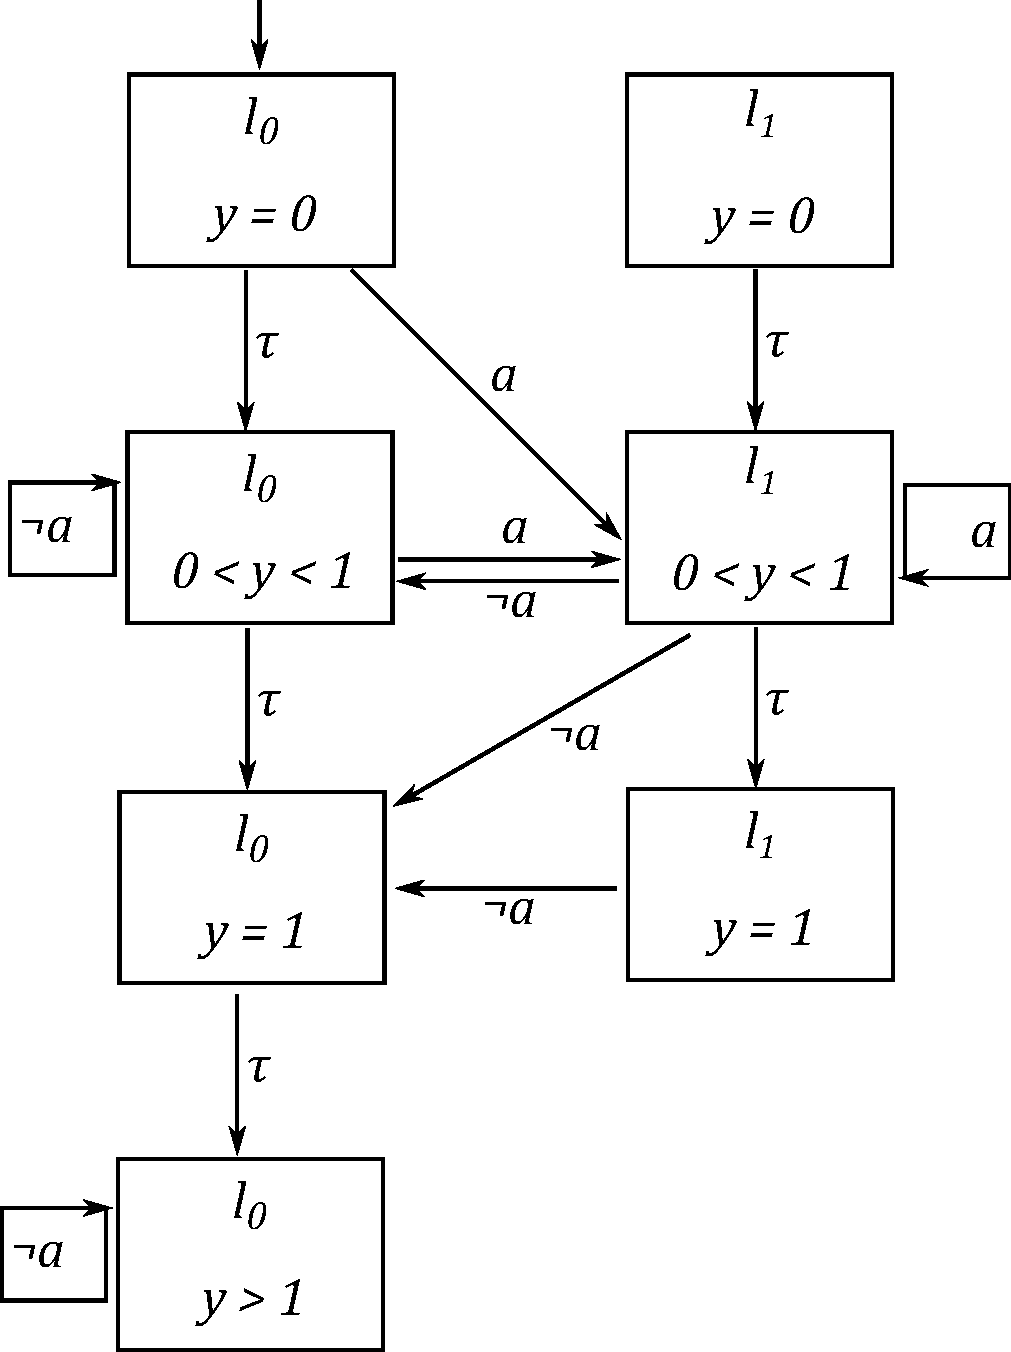
\includegraphics[width=0.5\textwidth]{images/region_graph.pdf}

\subsection*{2. Negation of $\varphi$ }
$\neg \varphi := \mathbf{G} \mathbf{F} \text{a}$

\subsection*{3. Büchi automaton $\mathcal{B}_{\neg \varphi}$}

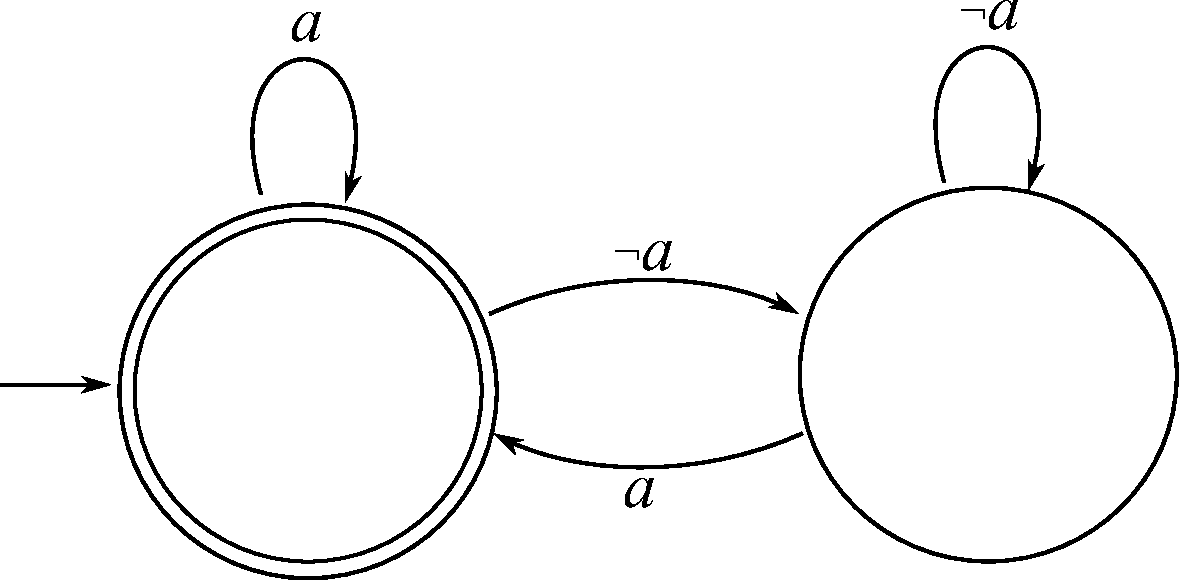
\includegraphics[width=0.3\textwidth]{images/buchi_aut.pdf}

\subsection*{4. Composition of Region Graph and Büchi Automaton}

\vspace*{14cm}

\subsection*{5. Loops in Composition Graph}

\newpage

\section*{Problem F3}
\subsection*{a)}


\subsection*{b)}


\subsection*{c)}


\subsection*{d)}



\section*{Problem F4}

\end{document}
